% \section{Подавление артефактов, вызванных наличием сильнопоглощающих включений}

\begin{frame}
\frametitle{Примеры артефактов}

\begin{columns}[t]
\column{.5\textwidth}
\centering
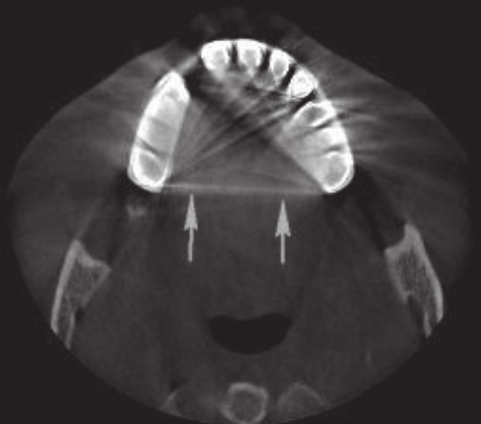
\includegraphics[height=0.35\textheight]{../Dissertation/images/part2_img/tooth_artifacts_med}\\ \vspace{5pt}
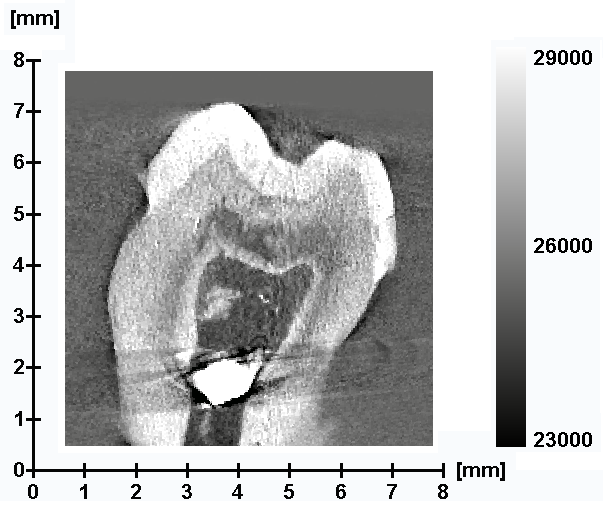
\includegraphics[height=0.55\textheight]{20180531_tooth_pb_slice}
\column{.5\textwidth}
\centering
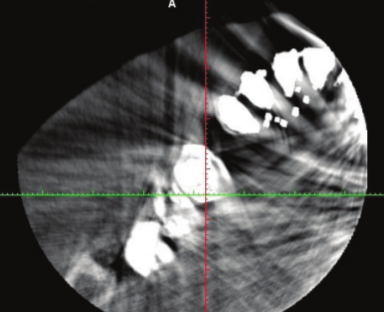
\includegraphics[height=0.35\textheight]{../Dissertation/images/part2_img/tooth_artifacts_med_3}\\ \vspace{5pt}
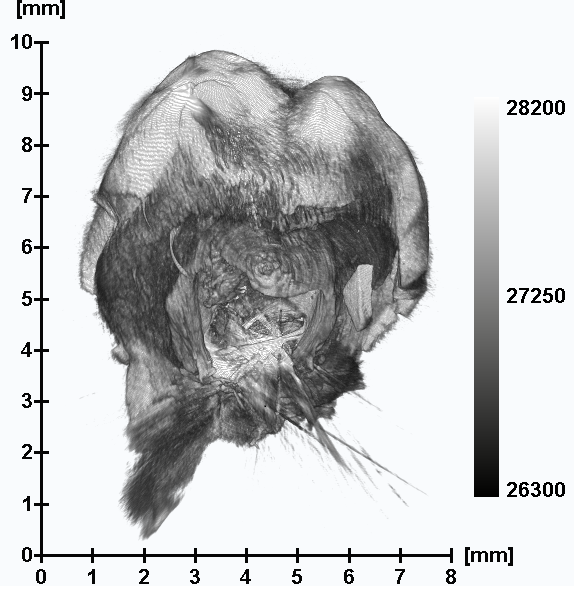
\includegraphics[height=0.55\textheight]{20180531_tooth_pb_vol}
\end{columns}

\end{frame}

\begin{frame}
\frametitle{Модель возникновения артефактов}
  \begin{itemize}[<+->]
%    \item при прохождении через сильнопоглощающие включения большая часть излучения поглощается
    \item пиксели детектора имеют некоторый порог активации $\delta_{\mathrm I min}$
    \item если пришедшая интетсивность $\mathrm I_{j} \leq \delta_{\mathrm I min}$, показание детектора будет неотличимо от уровня шума
%    \item при логарифмировании условие $\mathrm I_{j} \leq \delta_{\mathrm I min}$ переходит в 
    \begin{equation}
      \label{eq:thresh}
      p_j \geq \delta \left( = \ln \frac {\mathrm I_0}{\delta_{\mathrm I min}}\right)
    \end{equation}

    \item оптимизационная задача должна учитывать такие измерения особым образом
  \end{itemize}
\end{frame}



\begin{frame}
\frametitle{Учет пикселей с высоким поглощением}
Пусть $\mathbb J = \left\{ j | p_j \geq \delta \right\}$, то есть индексы пикселей, для которых выполнено условие (\ref{eq:thresh}).

С учетом пороговой активации, а так же неотрицательности функции $f$, оптимизационная задача будет иметь вид:


\begin{equation} \notag
  % \label{eq:quadprog_ineq}
  \begin{cases}
  \Norm{p - Wf} \rightarrow \min\limits_f & w.r.t \\
  \sum_i f_{i} \omega_{ij} > \delta, & \mbox{если } j \in \mathbb J \\
  f_{i} \geq 0 & \\
  \end{cases}
\end{equation}

\end{frame}


\begin{frame}
\frametitle{Квадратичное программирование}
\begin{itemize}
  \item оптимизация квадратичной функции на наборе линейных ограничений
  % \item частный случай выпуклой оптимизации
  \item требует обращения матрицы $W^{\mathrm T} W$. 
  \item для изображения 256х256 и 180 углов при использовании float64 такая матрица будет занимать порядка 12Гб
\end{itemize}

\end{frame}

\begin{frame}
\frametitle{Применение qp для малых размерностей}
\begin{columns}[T,onlytextwidth]
  \hspace*{-1cm}
\begin{column}{0.4\textwidth}
  \begin{figure}
    \centering
    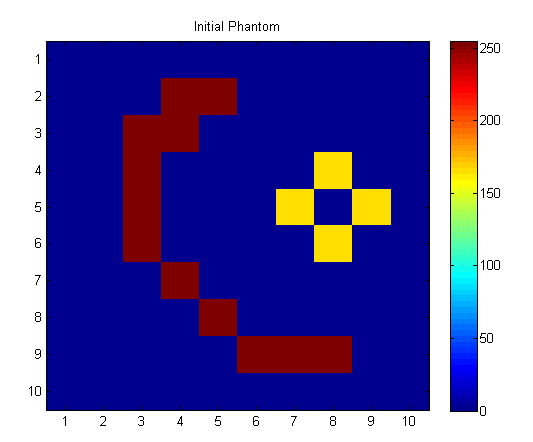
\includegraphics[width=\textwidth]{qp_phantom}
  \end{figure}
  фантом
\end{column}

\begin{column}{0.4\textwidth}
  \begin{figure}
    \centering
    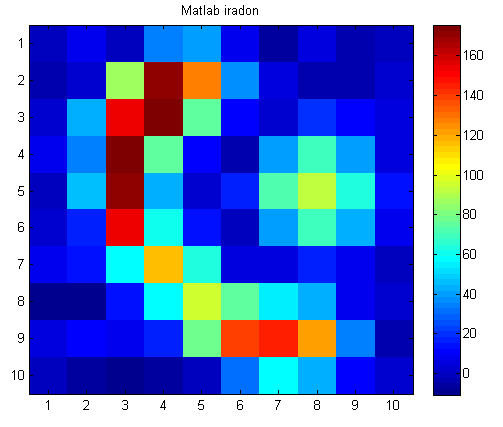
\includegraphics[width=\textwidth]{qp_fbp}
  \end{figure}
  matlab iradon (fpb)
\end{column}

\begin{column}{0.4\textwidth}
    \begin{figure}
    \centering
    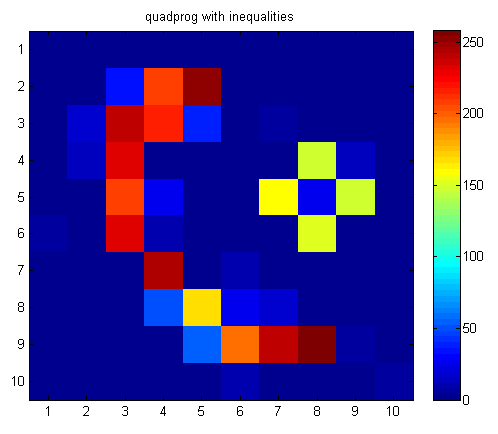
\includegraphics[width=\textwidth]{qp_qp_ineq}
  \end{figure}
  QP с ограничениями-неравенствами
\end{column}
\end{columns}

\end{frame}

\begingroup
\small
\begin{frame}
  \frametitle{Как повысить разрешение?}
  \begin{columns}[T, onlytextwidth]
  \hspace{-0.5cm}
  \begin{column}{0.5\textwidth}
    \underline{Метод мягких неравенств} \\ \vspace{0.5cm}
    Введем диагональную матрицу $\mathrm J \in \textup{diag}\{N N_\varphi\}$, такую что 
    $\mathrm J_{j} = \left\{1, \mbox{если}\ j \in \mathbb J, \mbox{иначе }\ 0\right\}$, а так же $\mathrm K = \mathrm E - \mathrm J$.


    \begin{equation} \notag
      \label{eq:soft-ineq}
      \begin{array}{lc}
      \Norm{K(Wf - p)}^2 & + \\
      \alpha \Norm{J(Wf - \delta)_{+}}^2  & \to \min\limits_f
      \end{array}
    \end{equation}
  \end{column}

  \begin{column}{0.5\textwidth}
    \underline{Метод барьерных функций} \\ \vspace{0.5cm}
    Заменим неравенства вида $g(x) \leq 0$ на аддитивные барьерные функции $-\frac 1 t \log{\left(-g(x)\right)}$.
    Начиная из ``внутренней''точки, будем минимизировать функционал, постепенно увеличивая t.
    $$
    \begin{array}{ccc}
      F_t(f) = & \Norm{Wf - p}^2 & + \\
     \frac 1 t \sum \left( -\log{\left(-g(x)\right)} \right) &\to \min\limits_f &
    \end{array}{ccc}
    $$

    Так же возможно ослабить ограничения, добавив переменные нежесткости $\xi$

  \end{column}
  \end{columns}
\end{frame}
\endgroup

\begin{frame}
\frametitle{Резульататы численного эксперимента}
\framesubtitle{к изображениям применена гамма-коррекция}

\begin{figure}
  \centering
  \vspace{-0.3cm}
  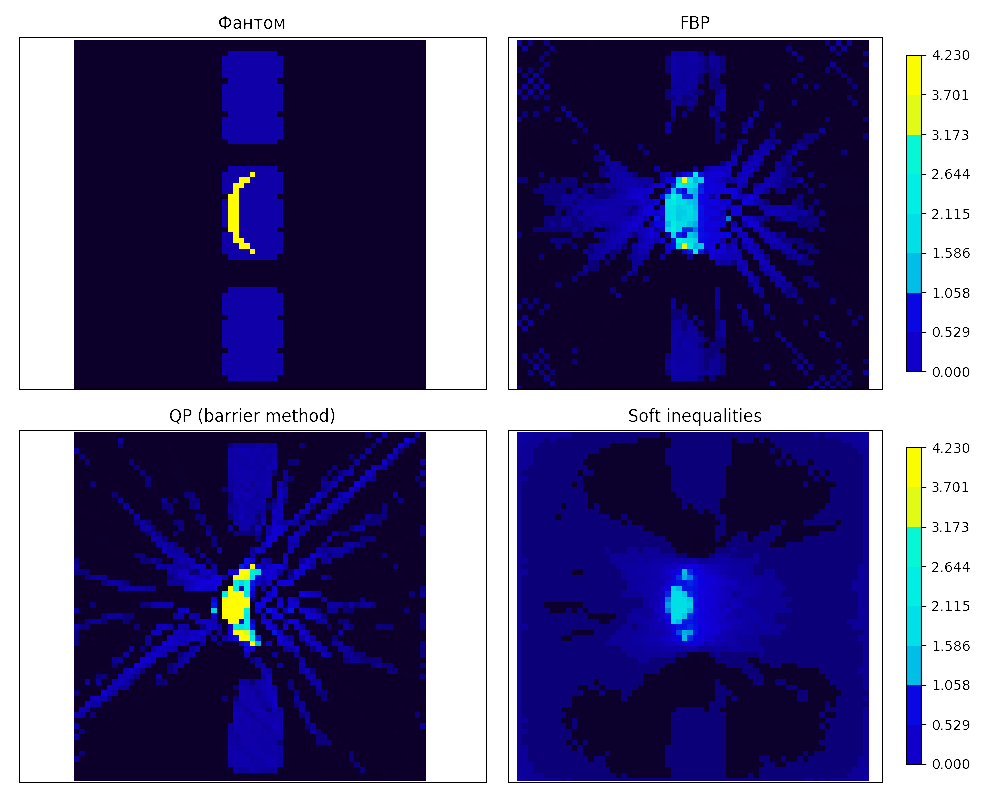
\includegraphics[height=0.7\textheight]{qp_foursome}
  \caption{сравнение реконструкции различными методами}
  \label{fig:sample}
\end{figure}

\end{frame}

\begin{frame}
\frametitle{Резульататы численного эксперимента}
\framesubtitle{к изоюражениям применена гамма-коррекция}

\begin{figure}
  \centering
  % \vspace{-0.3cm}
  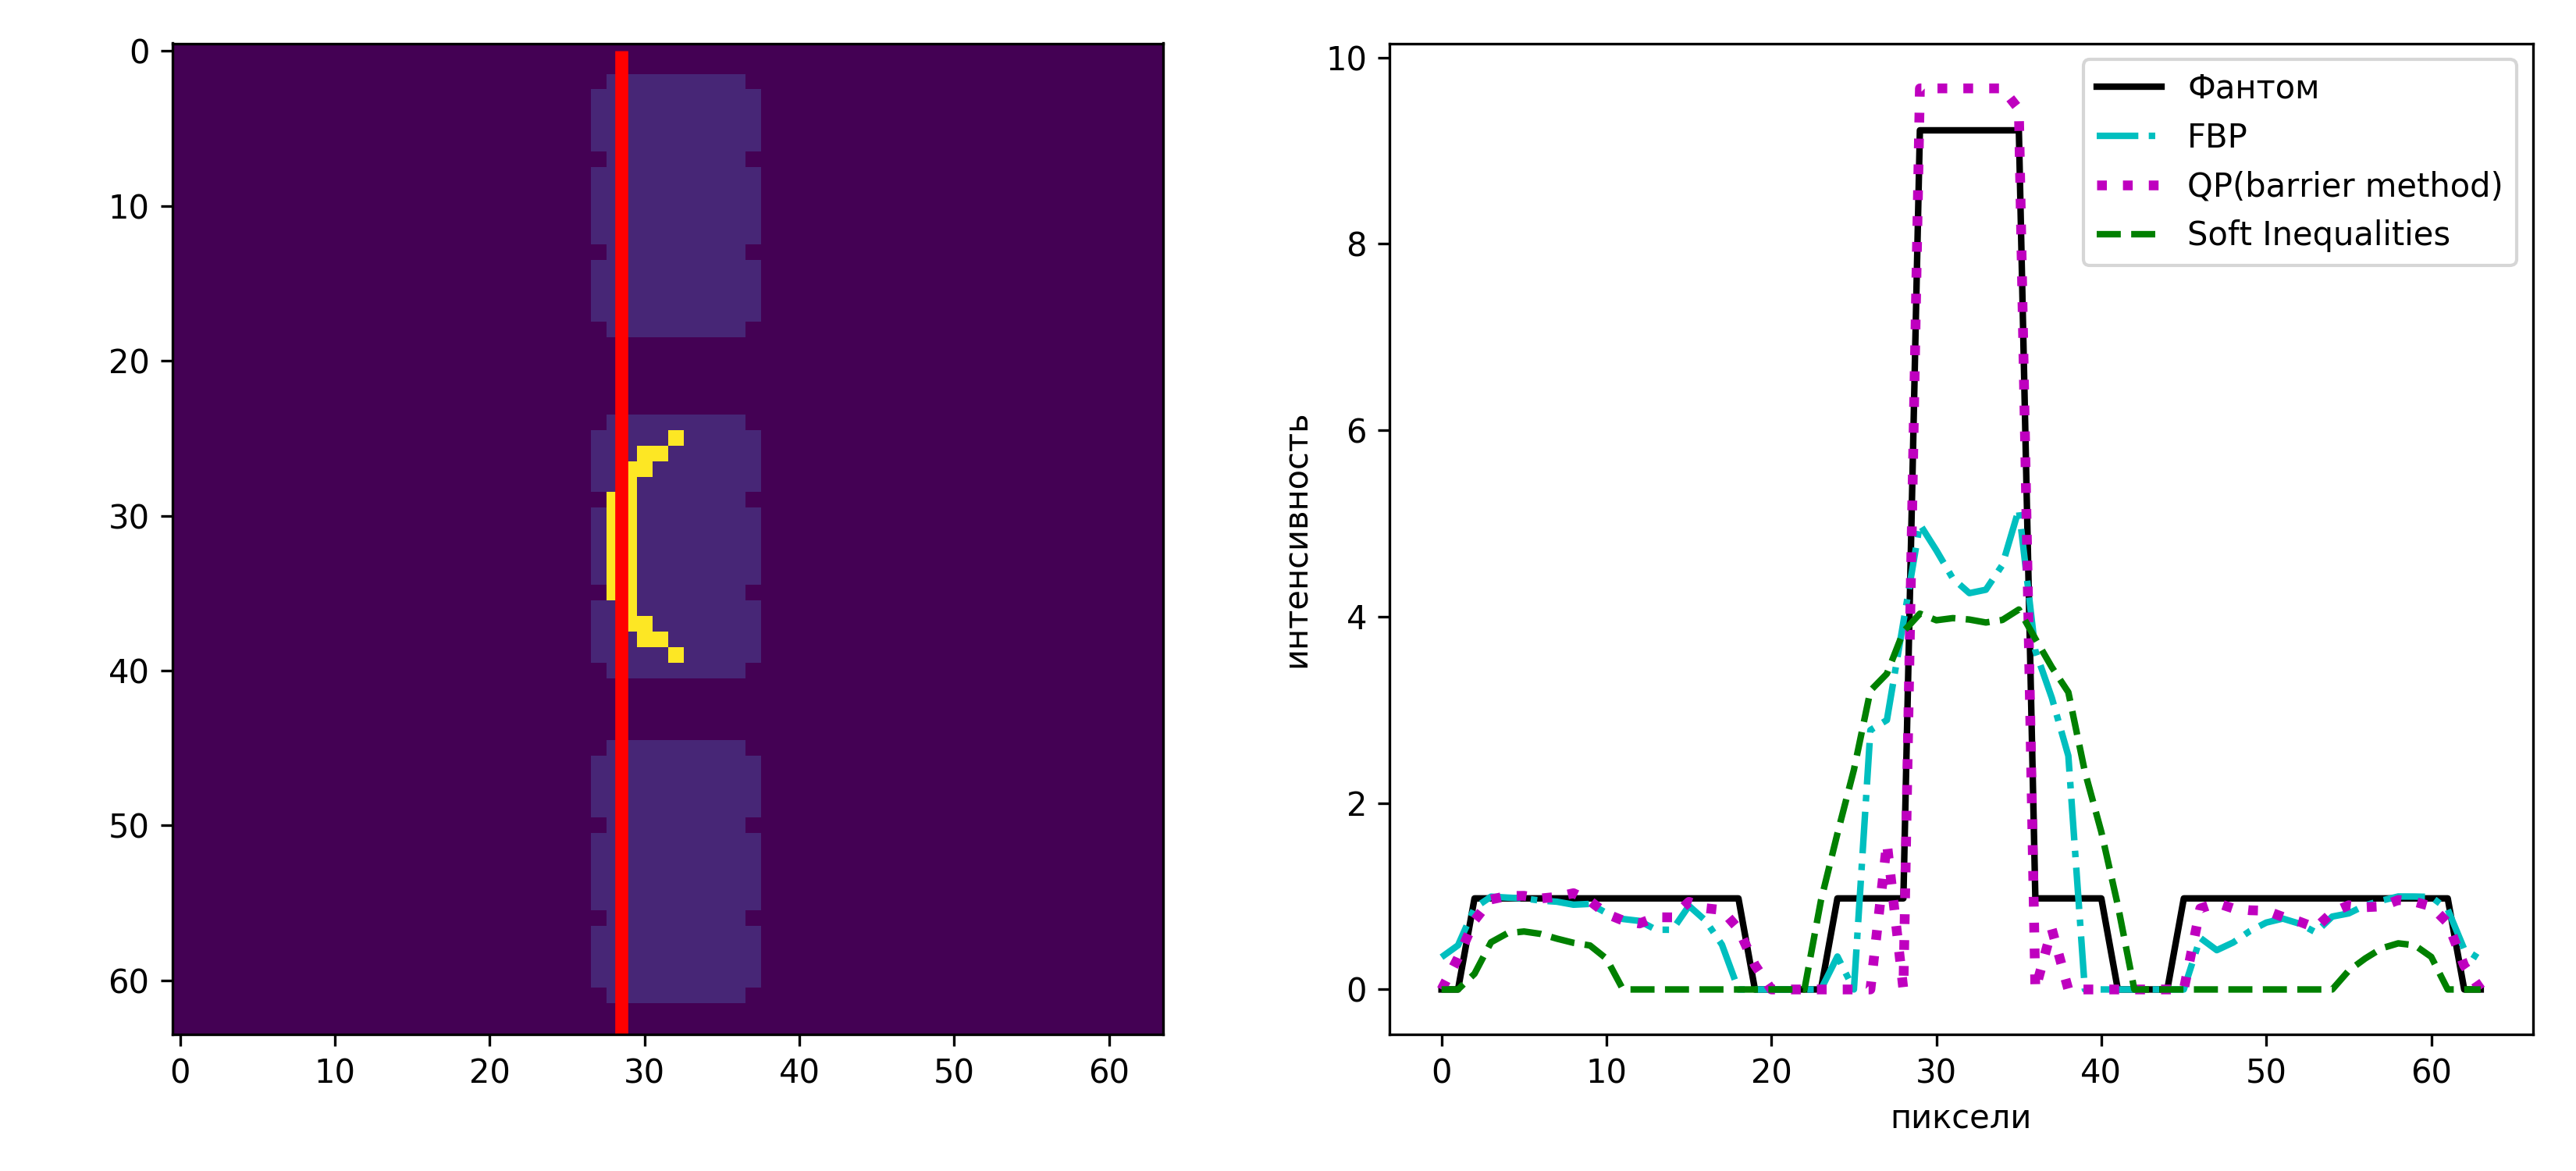
\includegraphics[width=\textwidth]{qp_cs_x28}
  \caption{кросс-секции реконструкций}
  \label{fig:sample}
\end{figure}

\end{frame}


\begin{frame}
\frametitle{Метод мягких неравенств}
\framesubtitle{реконструкция экспериментальных данных}

\centering
\vspace{-0.3cm}
\begin{columns}
\vspace{-1.2cm}
\begin{column}{0.3\textwidth}
\begin{figure}
    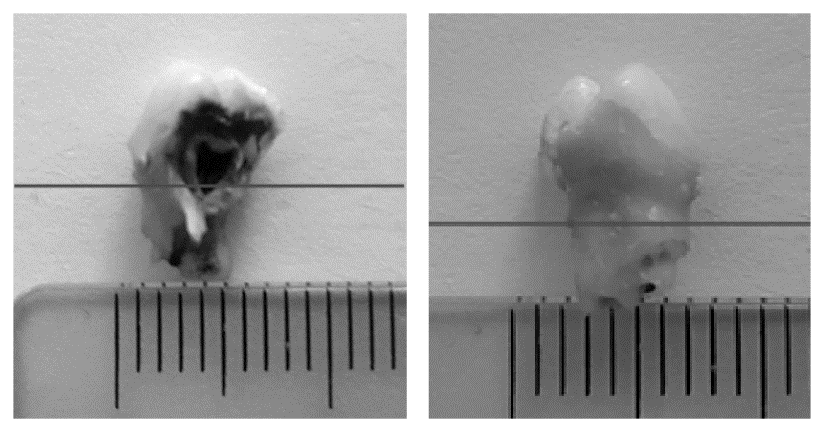
\includegraphics[width=1\textwidth]{zub_photo}
    \caption{Образец: молочный зуб с включением из свинца}
\end{figure}
\end{column}

\begin{column}{0.85\textwidth}
\vspace{-0.3cm}
\begin{figure}
    \centering
    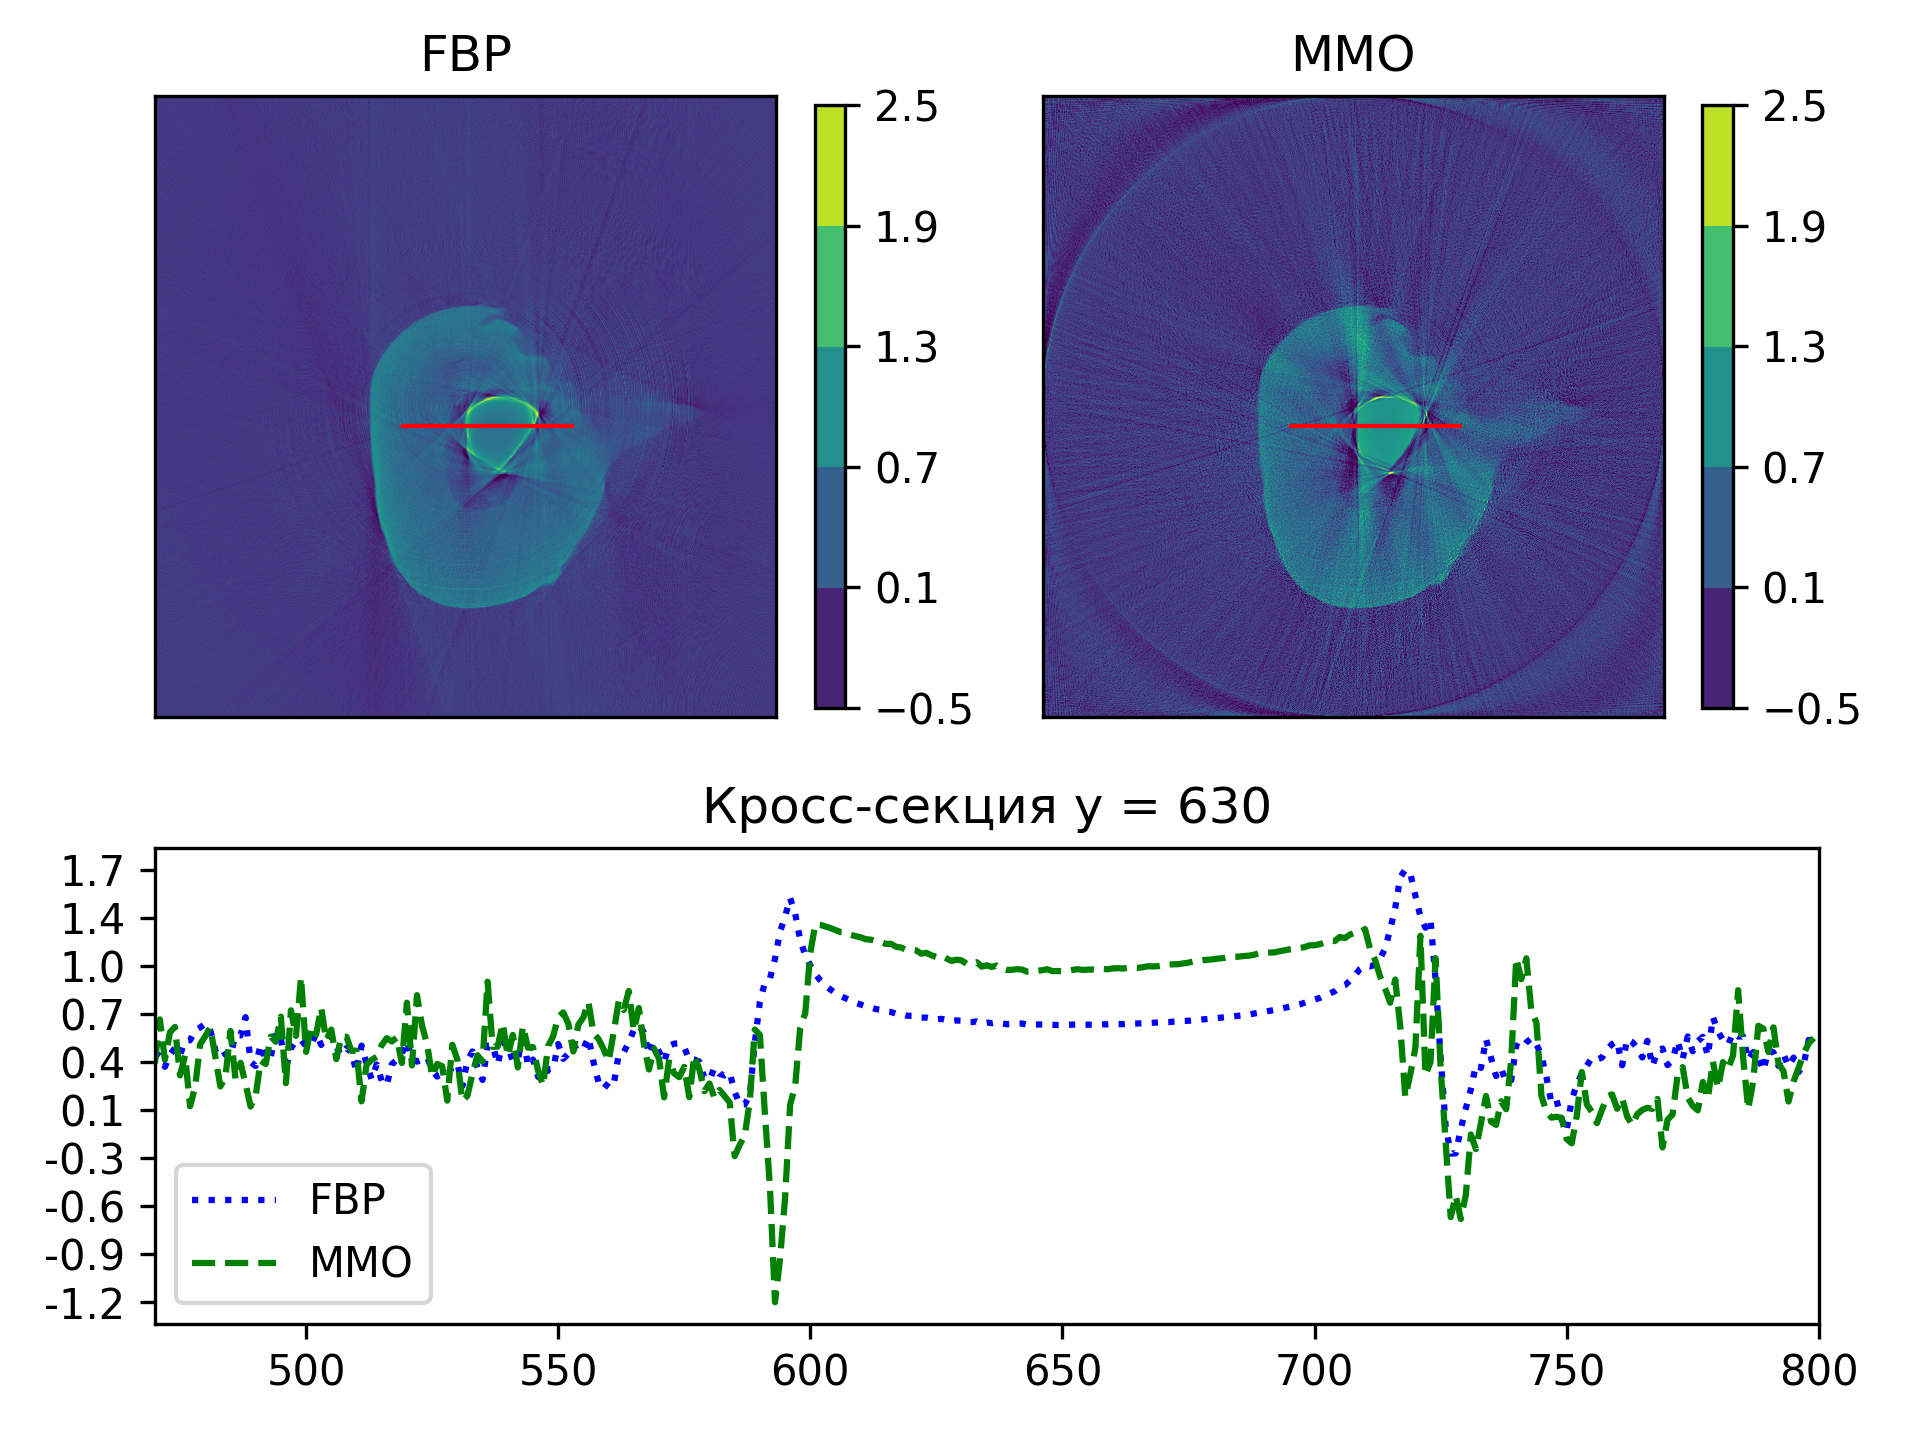
\includegraphics[width=\textwidth]{../Dissertation/images/part2_img/pb_big__fbp_vs_soft__cs__viridis} \\

    \caption{Результаты восстановления}
    \label{fig:fbp_vs_soft__zub}
\end{figure}
\end{column}
\end{columns}

\end{frame}

\begin{frame}
\frametitle{Выводы}
\begin{itemize}
  \item Подход, основанный на ограничениях-неравенствах, позволяет улучшить качество восстановления в рамках предложенной модели
  \item На модельных данных метод барьерных функций показывает лучшее, чем метод мягких ограничений или метод FBP, качество восстановления
  \item На реальных экспериментальных измерениях показано, что метод мягких ограничений позволяет добиться локально-постоянной интенсивности сильнопоглощающего включения
  \item Публикации \cite{ecms2015Chukalina, icmv2015Chukalina,trudi_isa_2018}
\end{itemize}
\end{frame}